\chapter{Containerization with Docker}
\label{cha:containerization-docker}
Docker \cite{Docker2018} is a tool for creating, provisioning and interacting with Linux Containers (LXC). LXC are a lightweight version of virtualization which does not have the resource impact of a full virtualization such as OS virtualization. The differences of LXC an hypervisor based virtualization a re covered in section \ref{sec:docker-virtualization-vs-containerization}. Docker has become very popular over the past years, due to the fact, that it made it possible to easily work with LXC. Docker relies strongly on the principles of IaC which has been discussed in chapter \ref{cha:iac}. When using Docker, Linux containers are often referred as Docker containers.

Containerization is a key factor in cloud based development, because applications normally are packaged in images and run as containers on the cloud platform. Containerization provides features for a fast, effortless and consistent way of running applications in the cloud, which are discussed in section \ref{sec:docker-need-for-containerization}.

\section{The need for Containerization}
\label{sec:docker-need-for-containerization}
Containerization is a key factor for cloud platforms such as PaaS, where each application runs in its own isolated environment, called a container. A container is an instance of an image, which represents the initial state of an application. A virtual machine represents a full blown OS, where the OS provides a kernel, which is emulated on the host OS by the hypervisor. A hypervisor is a software which can create, run and manage virtual machines. A container uses the kernel provided by the host OS and therefore does not perform any emulation. A container does not represent a full blown OS, but still provides features such a networking, storage and the OS file system.  

Containers are faster to create, deploy and easier to manage than virtual machines. Nevertheless, cloud platforms use virtualization for managing their infrastructure, where the containers run on the provisioned virtual machines. The usage of containers compared to the usage of virtual servers can reduce costs for hosting applications. Enterprises can profit from hosting their applications of containers in several ways. Applications hosted in containers need lees resources than applications hosted in virtual servers, because there is no virtualized OS. The creation, deployment and startup of containers are faster, because only the isolated process needs to be started and not a full blown OS. Docker is well supported by Integrated Development Environments (IDEs), which provide support for creating Docker image definitions (Dockerfiles) and provisioning of Docker Containers on a local or remote environment.

When enterprises have applied IaC to their infrastructure life cycle, then the next logical step is to integrate their applications into IaC as well. Applications hosted in containers profit from the IaC principles immutability, reproducibility, repeatability and consistency. Therefore, Docker strongly relies on IaC and provides tooling for automating creation and deployment of docker containers, which is used by PaaS platforms such as Openshift. With Docker, developers define the hosting environment for their applications now and not system administrators anymore. Nevertheless, developers can profit from the deep Linux knowledge of system administrators, to define the Docker images efficiently, to keep them small and secure. 

\section{Docker}
\label{sec:docker}
This section covers Docker, which is the most popular tool to work with LXC. Docker is open source but also provides an enterprise support if needed. The core part of the Docker technology is the Docker Engine which is covered in section \ref{sec:docker-engine}. the Docker Engine is the part of the Docker technology that actually runs the containers. The Docker Images are managed in a so called Docker registry \cite{DockerRegistry2018}, which is a repository for Docker images. The most popular Docker registry is Docker Hub \cite{DockerRegistry2018}, which is a free service, where anyone can provides Docker images.

\subsection{Docker Engine}
\label{sec:docker-engine}
Figure \ref{fig:docker-engine} illustrates the Docker Engine hosted on a Linux OS. The Docker Engine is build by layers, where each layer communicates with the layer beneath and the Docker Engine represent the core of the Docker architecture. 

\begin{figure}[htbp]
	\centering
	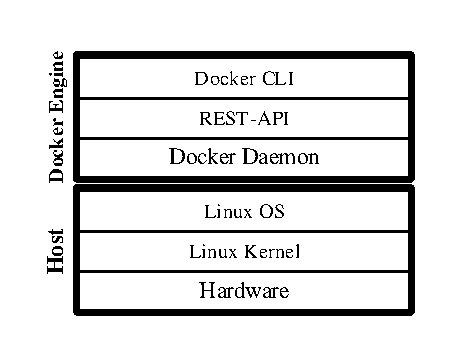
\includegraphics[scale=0.8]{images/docker-engine.pdf}
	\caption{Docker Engine Architecture}
	\label{fig:docker-engine}
\end{figure} 

\mysubsubsection{Docker Damon and REST-API}
\label{sec:docker-daemon}
The docker daemon represents the background process on a Linux OS, which creates, runs and manages the Docker Containers on the Docker host. A connection to the Docker daemon can be established via a Unix socket or a network interface, depending on the configuration of the Docker daemon. If the Docker daemon is exposed via a network interface, then it is recommended to secure the connection with client certificate authentication.

\mysubsubsection{Docker Command Line interface (CLI)}
The Docker Engine provides a CLI for interacting with the Docker daemon via a Linux shell. The Docker CLI itself communicates with the Docker daemon via the exposed REST-API. This is the most common way to interact with a Docker daemon. The Docker CLI provides commands for creating Docker Images and Containers and for provisioning the Docker Containers on the Docker Host.

\mysubsubsection{Docker Images}
\label{sec:docker-images}
Docker images are defined via Dockerfiles, which contains instructions how to build the Docker image. A Docker image consists of layers, where each layer represents a state of the file system, produced by a Dockerfile instruction. Each layer is immutable and and any change on the file system produces a new layer. Docker Images are hierarchical and can inherit from another image, which is then called base image. Docker images support only single inheritance and the base image is defined via the FROM instruction as the first instruction in the Dockerfile. Docker image names have the structure \mentionedtext{[namespace]/[name]:[version]} e.g. \mentionedtext{library/openjdk:8-alpine}.

\mysubsubsection{Docker Containers}
\label{sec:docker-containers}
A Docker container is an instance of a Docker image, where a new layer is appended, which contains all changes made on the file system by the running process within the Docker container. When the container is deleted, then the appended layer gets deleted as well and all made changes on the file system are lost. A Docker container keeps running as long as the contained foreground process is running. Without a foreground process the Docker container stops immediately after it was started. The process running in the container is isolated from other processes, as well is the file system, the process has access to.

\subsection{Docker Architecture}
\label{sec:docker-architecture}
The Docker architecture is a client server architecture, therefore the communication to the Docker daemon is done via the REST-API. 

\begin{figure}[htbp]
	\centering
	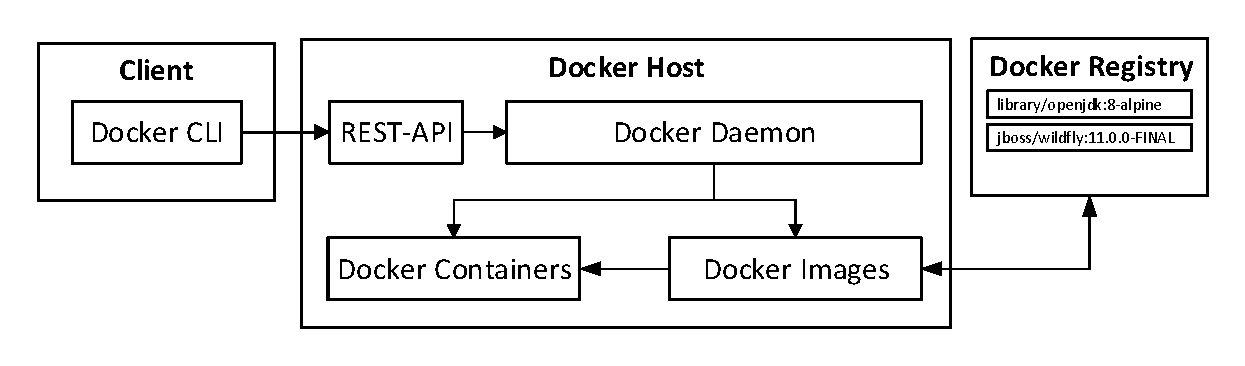
\includegraphics[scale=0.7]{images/docker-architecture.pdf}
	\caption{Docker Architecture}
	\label{fig:docker-enginarchitecture}
\end{figure} 

\section{Virtualization vs. Containerization}
\label{sec:docker-virtualization-vs-containerization}
Before LXC, the industry made heavy use of operating system (OS) virtualization to isolate their environments and applications. A virtual machine is managed by a hypervisor, which is software, which can create, run and manage virtual machines. The virtual machine provides resources such as network and storage for the application, which is managed by the virtualized OS. Nevertheless, an virtual machine represents a full blown OS, which itself has a resource need which adds to the resource needs of the hosted application.

LXC on the other hand is a kernel technology, which provides resources such as network and storage to the application as well, but without the need of virtualized OS. 